\subsection{Student Pages}

\noindent These pages support student-side interactions, from finding tutors to booking sessions and tracking progress.

\subsubsection{Student Dashboard}

\noindent The student dashboard serves as the central hub for students, providing a comprehensive overview of their academic progress, registered courses, upcoming sessions, and mentor information.

\begin{figure}[H]
    \centering
    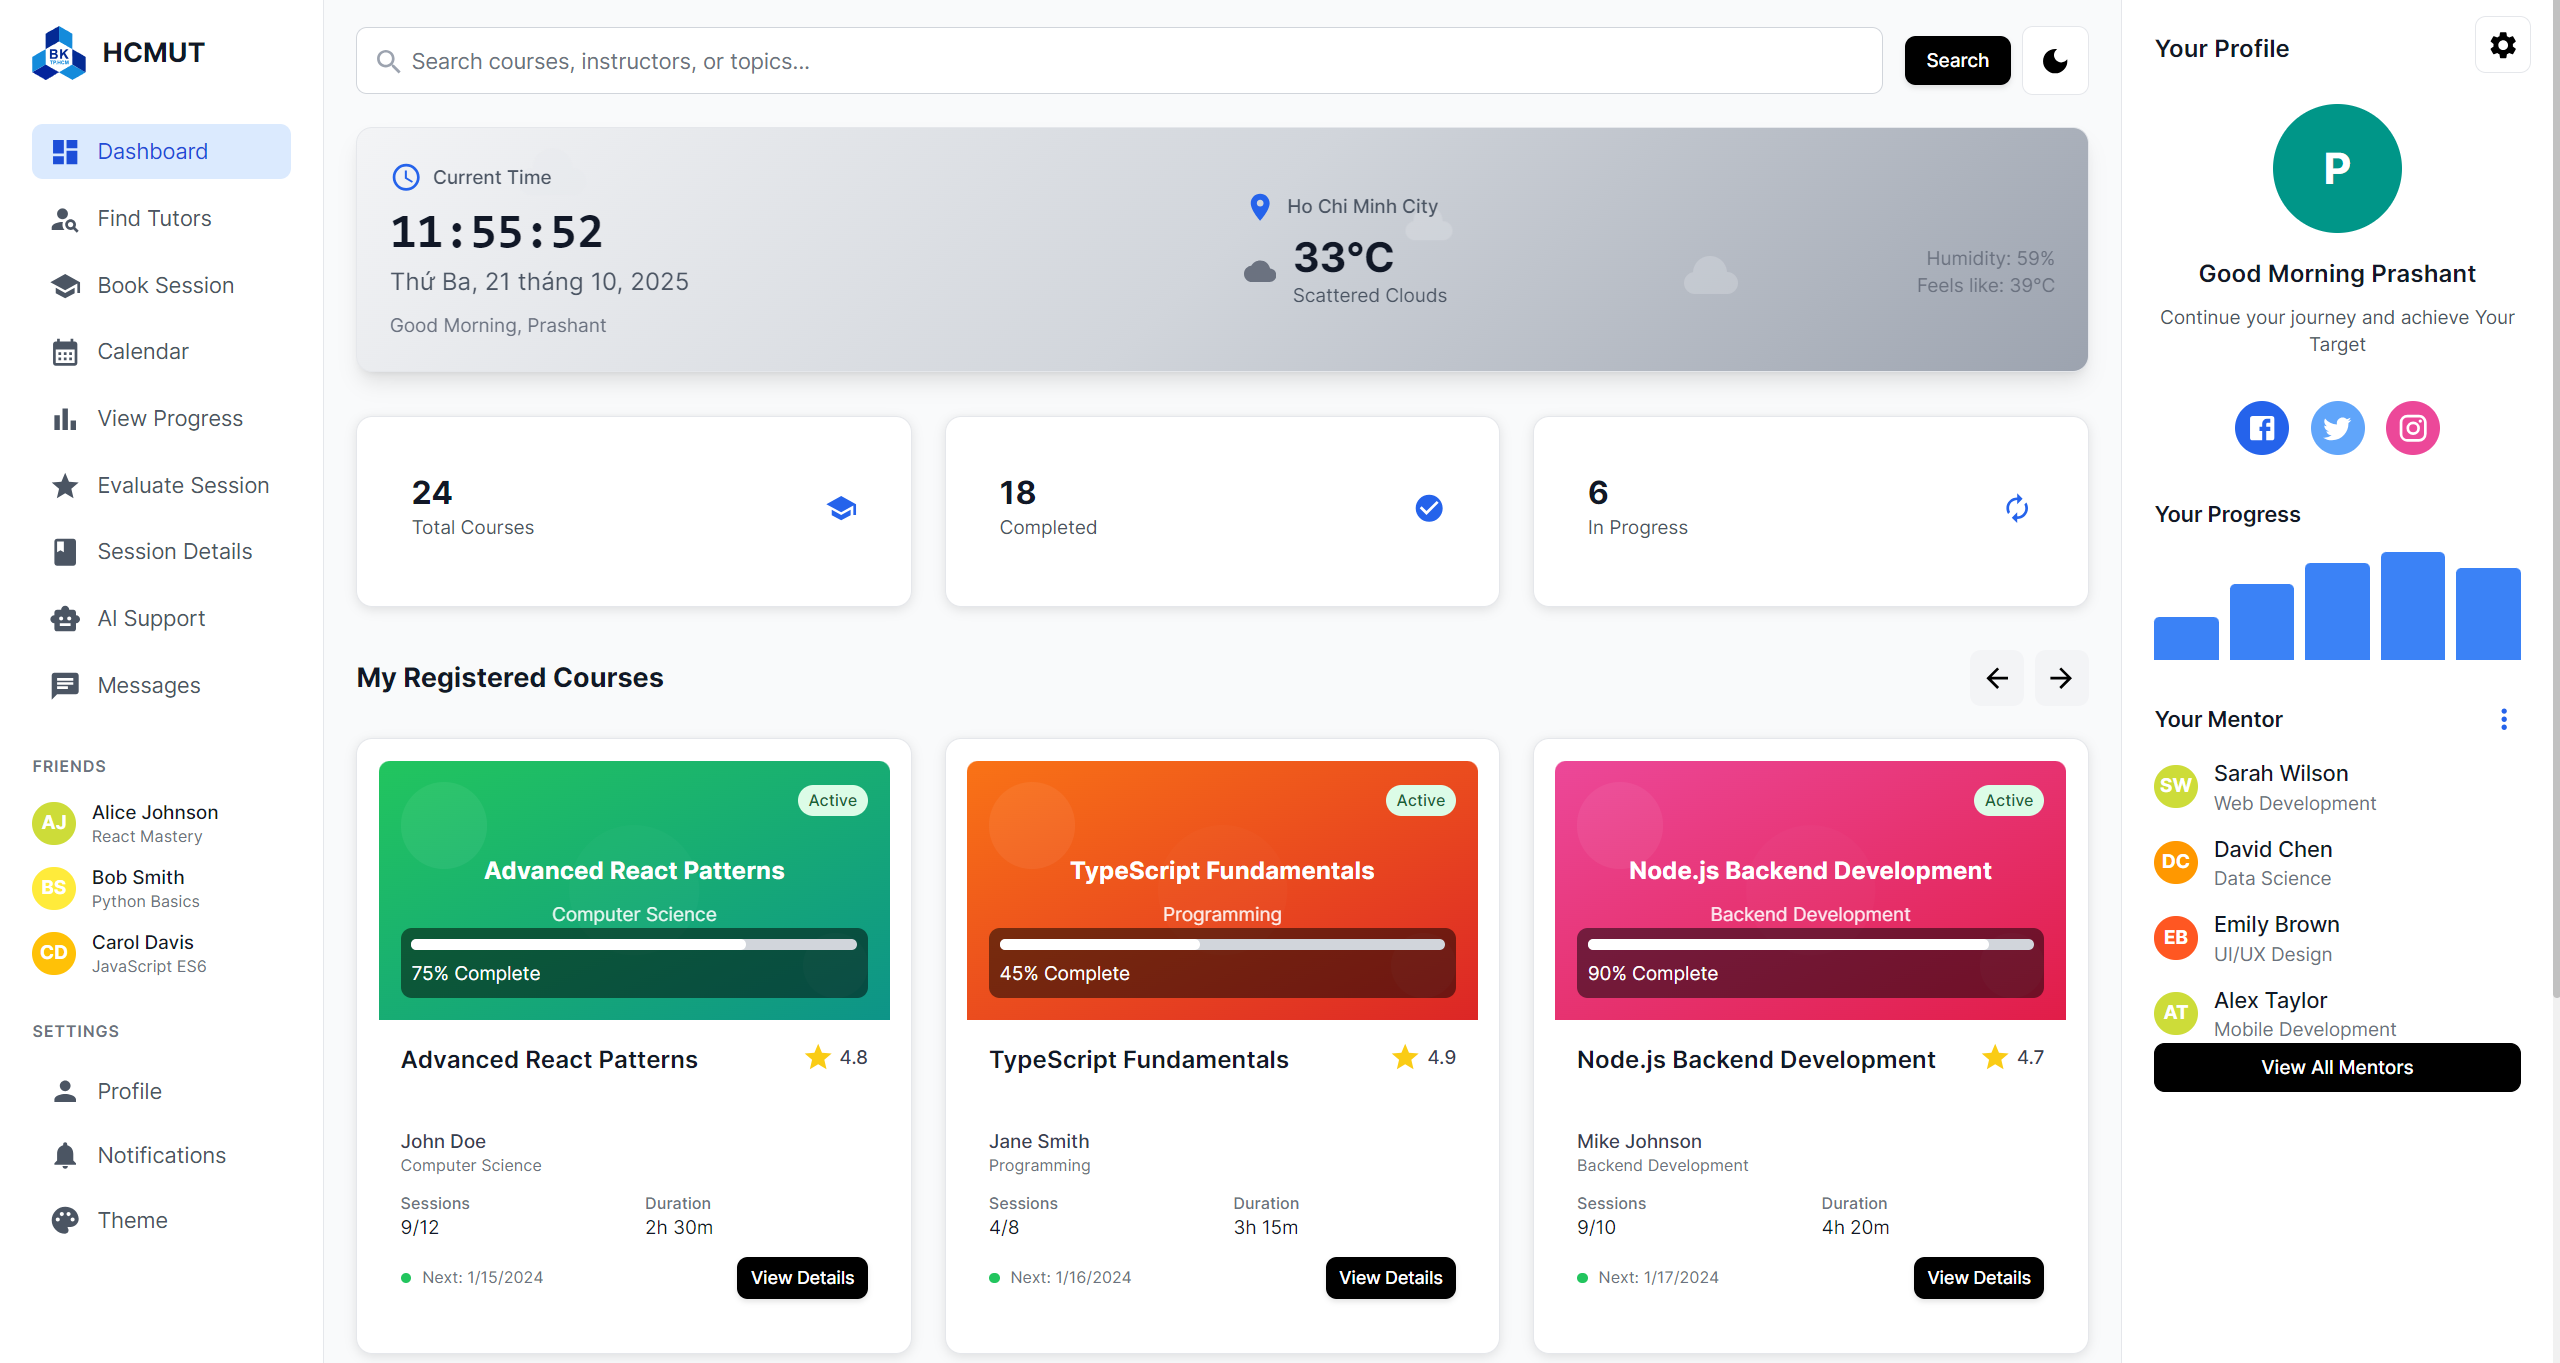
\includegraphics[width=\textwidth]{graphics/chapter2/student/student_dashboard_overall.png}
    \caption{Student Dashboard Overview}
    \label{fig:student_dashboard_overall}
\end{figure}

\paragraph{General Overview}
The dashboard features a three-column layout: left navigation sidebar, central content area, and right profile panel.

\subsubsection{Search Tutors}

\noindent The "Search Tutors" page allows students to find and connect with suitable tutors based on various criteria. It provides filtering options and displays available tutors with their profiles and session booking capabilities.

\begin{figure}[H]
    \centering
    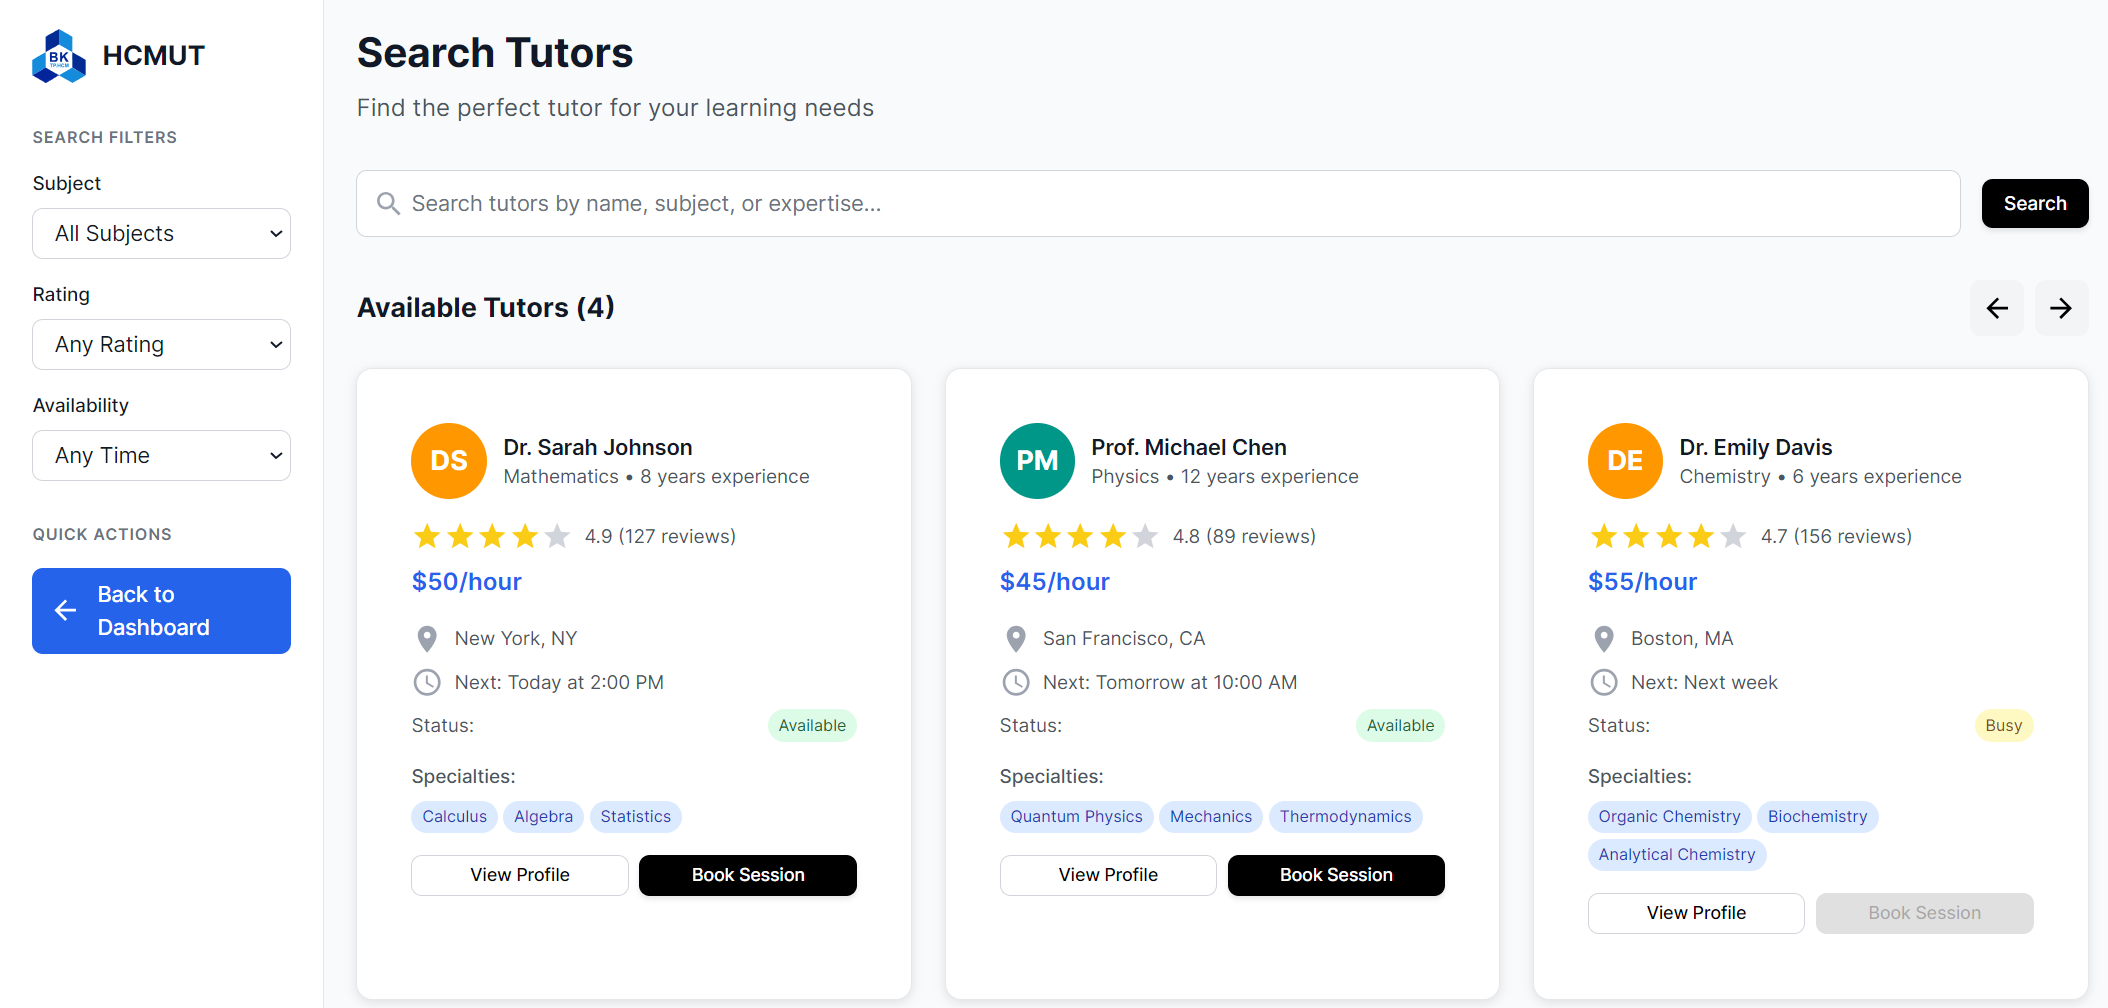
\includegraphics[width=\textwidth]{graphics/chapter2/student/search_tutors_overall.png}
    \caption{Search Tutors Page Overview}
    \label{fig:search_tutors_overall}
\end{figure}

\paragraph{General Overview}
The page features a two-column layout: a left sidebar for search filters and a main content area displaying tutor results.

\subsubsection{Book Session}

\noindent The "Book Session" page guides students through a four-step process to schedule a tutoring session. It provides a clear, structured interface to select a tutor, choose a date and time, confirm session details, and proceed with payment.

\begin{figure}[H]
    \centering
    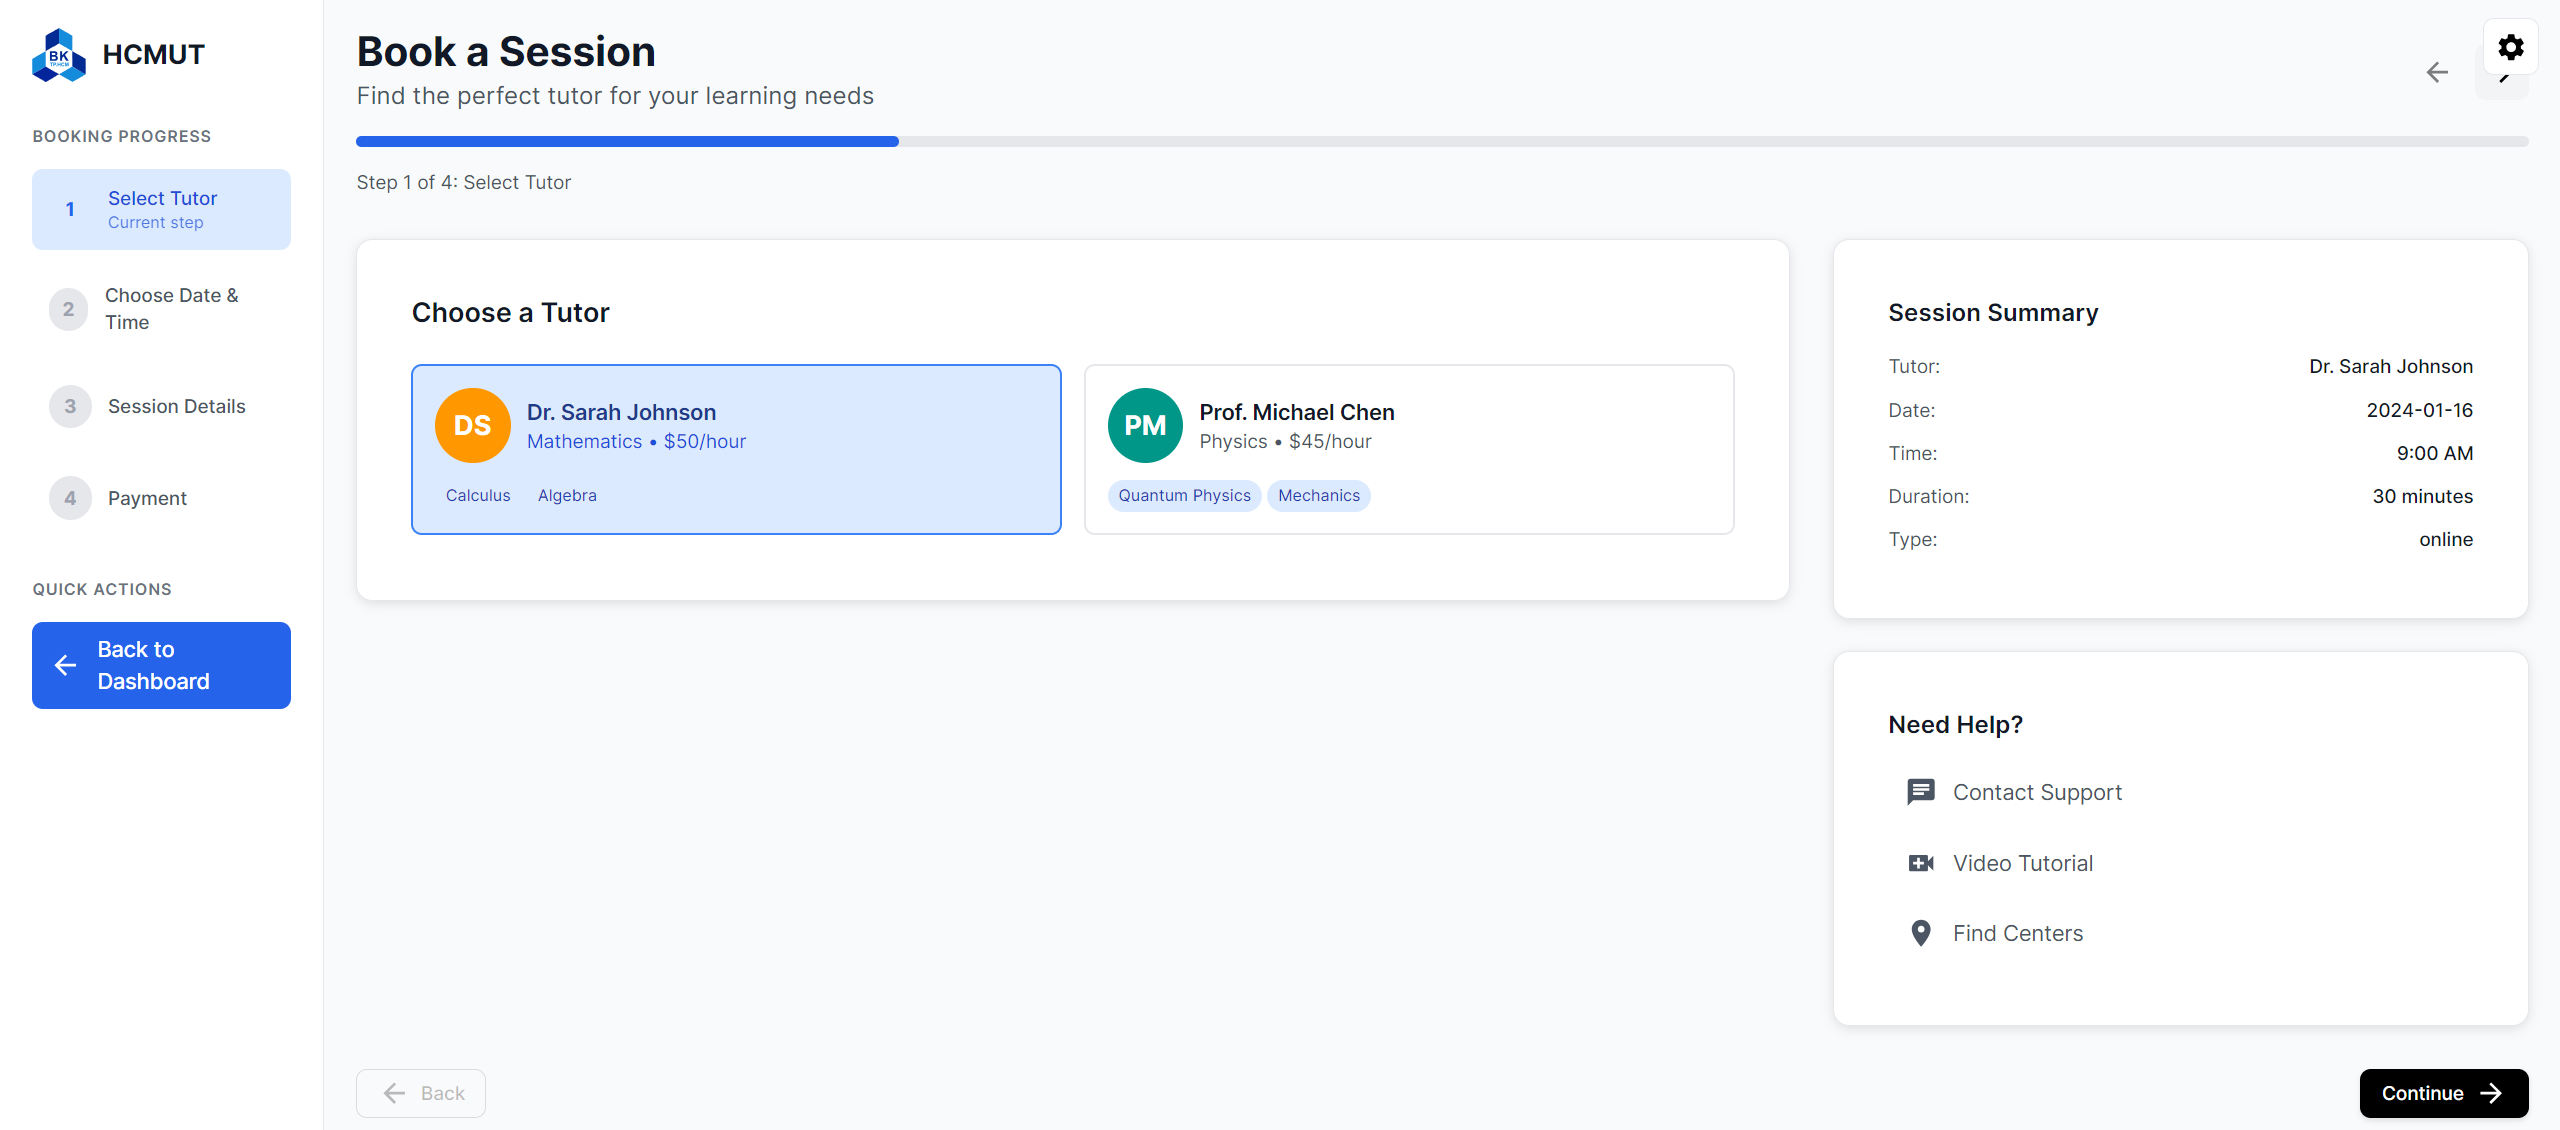
\includegraphics[width=\textwidth]{graphics/chapter2/student/book_session_step1.png}
    \caption{Book Session - Step 1: Select Tutor}
    \label{fig:book_session_step1}
\end{figure}

\paragraph{Step 1: Select Tutor}
The first step allows students to choose from available tutors. The page features a three-column layout with booking progress on the left, tutor selection in the center, and session summary on the right. Students can view tutor profiles, rates, and specialties before making their selection.

\begin{figure}[H]
    \centering
    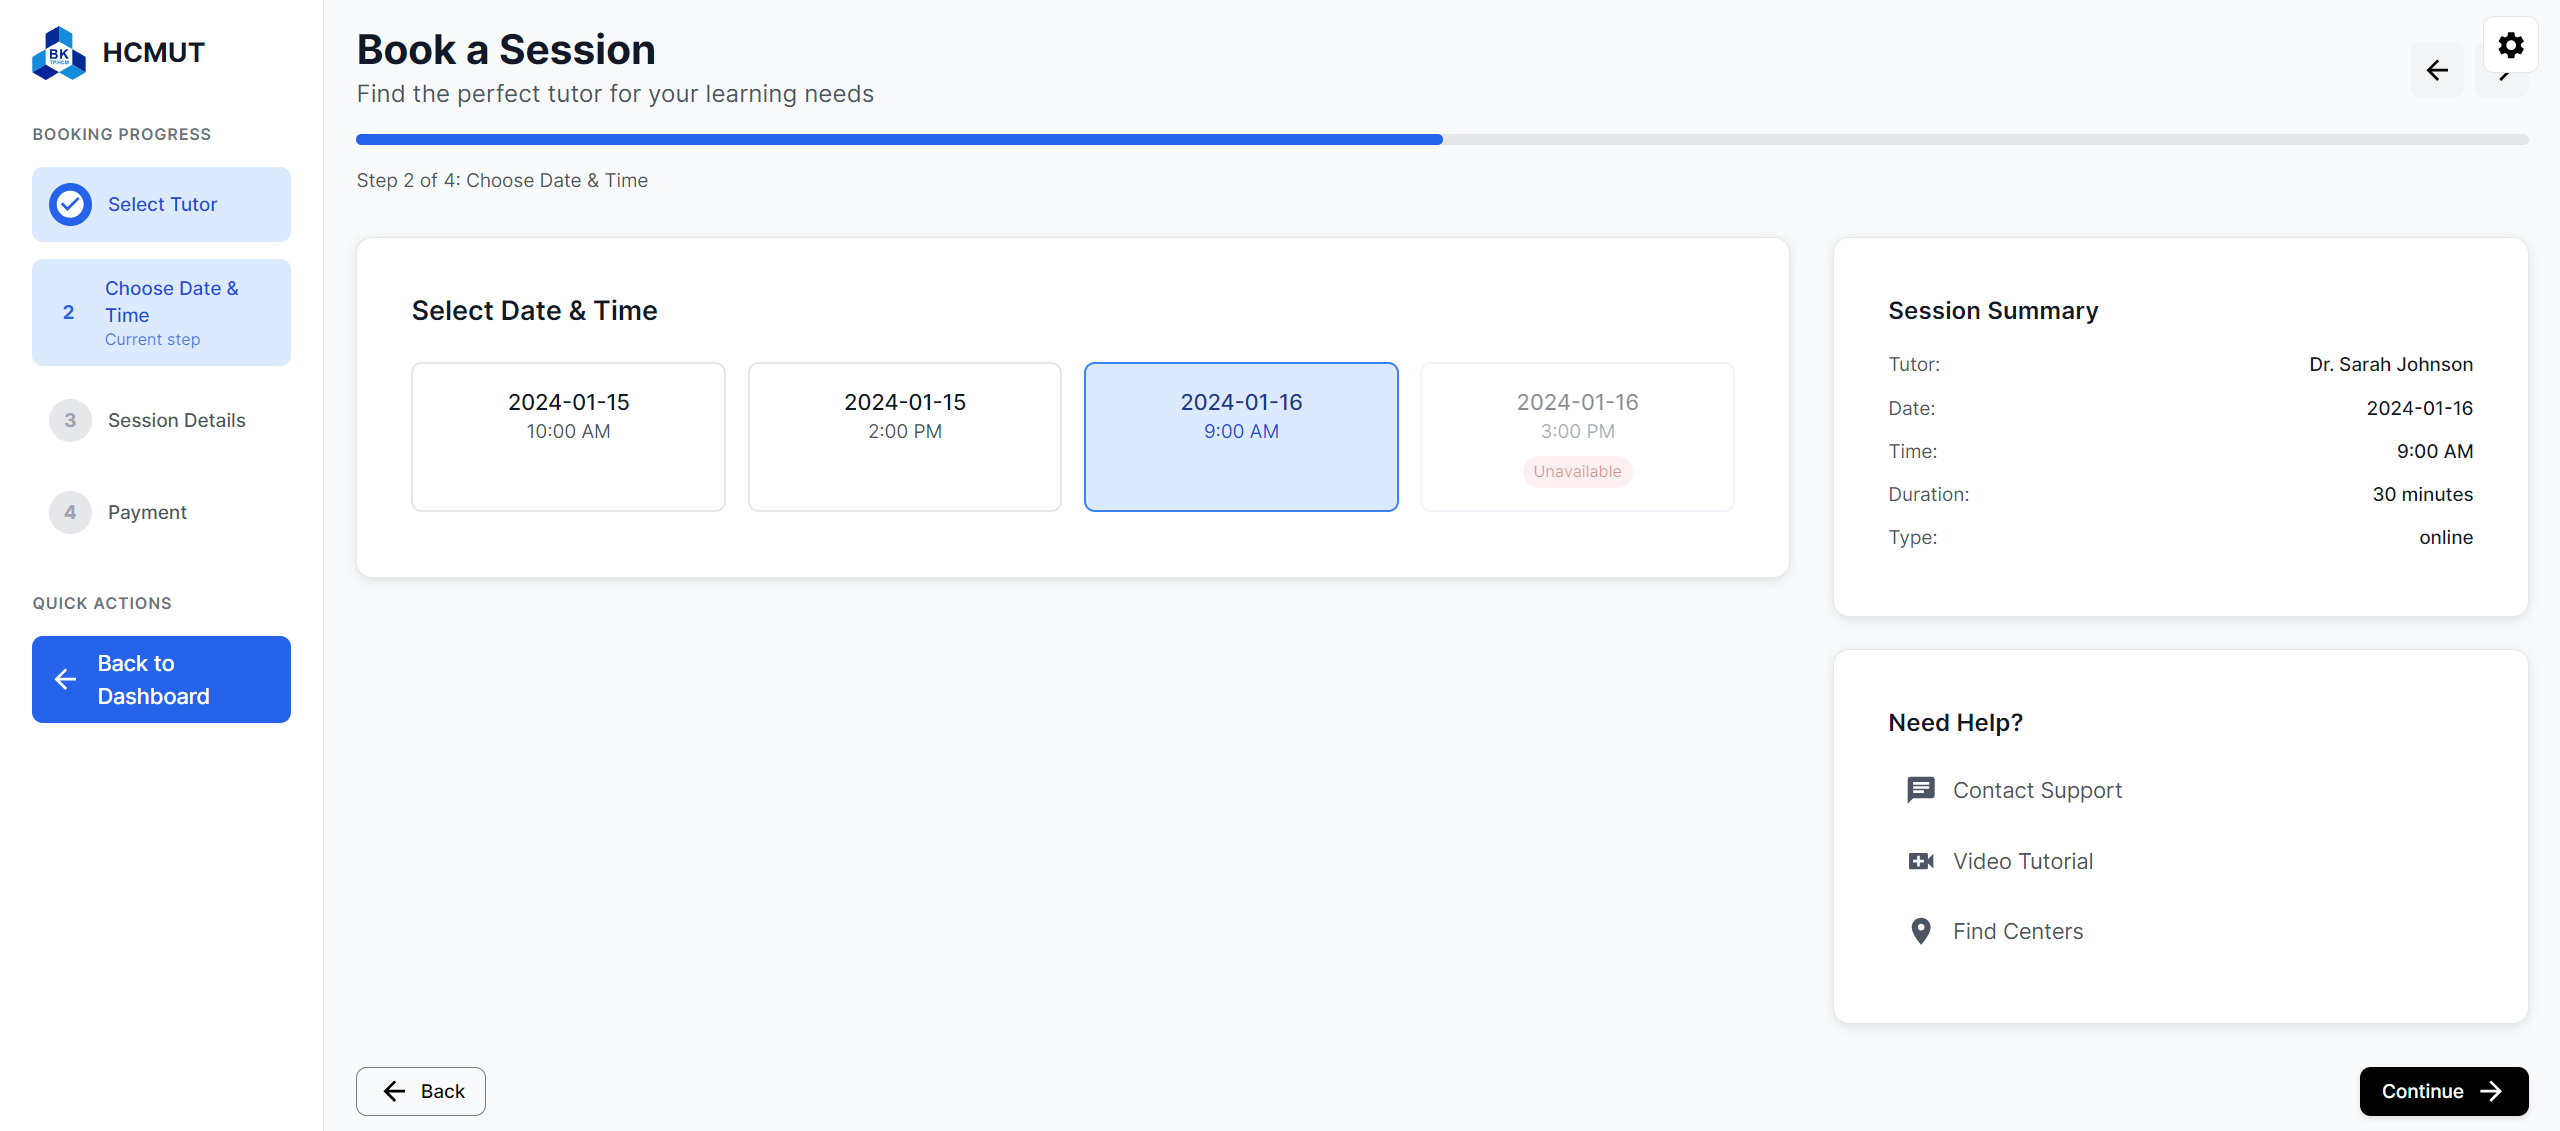
\includegraphics[width=\textwidth]{graphics/chapter2/student/book_session_step2.png}
    \caption{Book Session - Step 2: Choose Date \& Time}
    \label{fig:book_session_step2}
\end{figure}

\paragraph{Step 2: Choose Date \& Time}
The second step enables students to select their preferred date and time slot. Available time slots are displayed with clear indicators for availability, while unavailable slots are grayed out. The selected slot is highlighted in blue.

\begin{figure}[H]
    \centering
    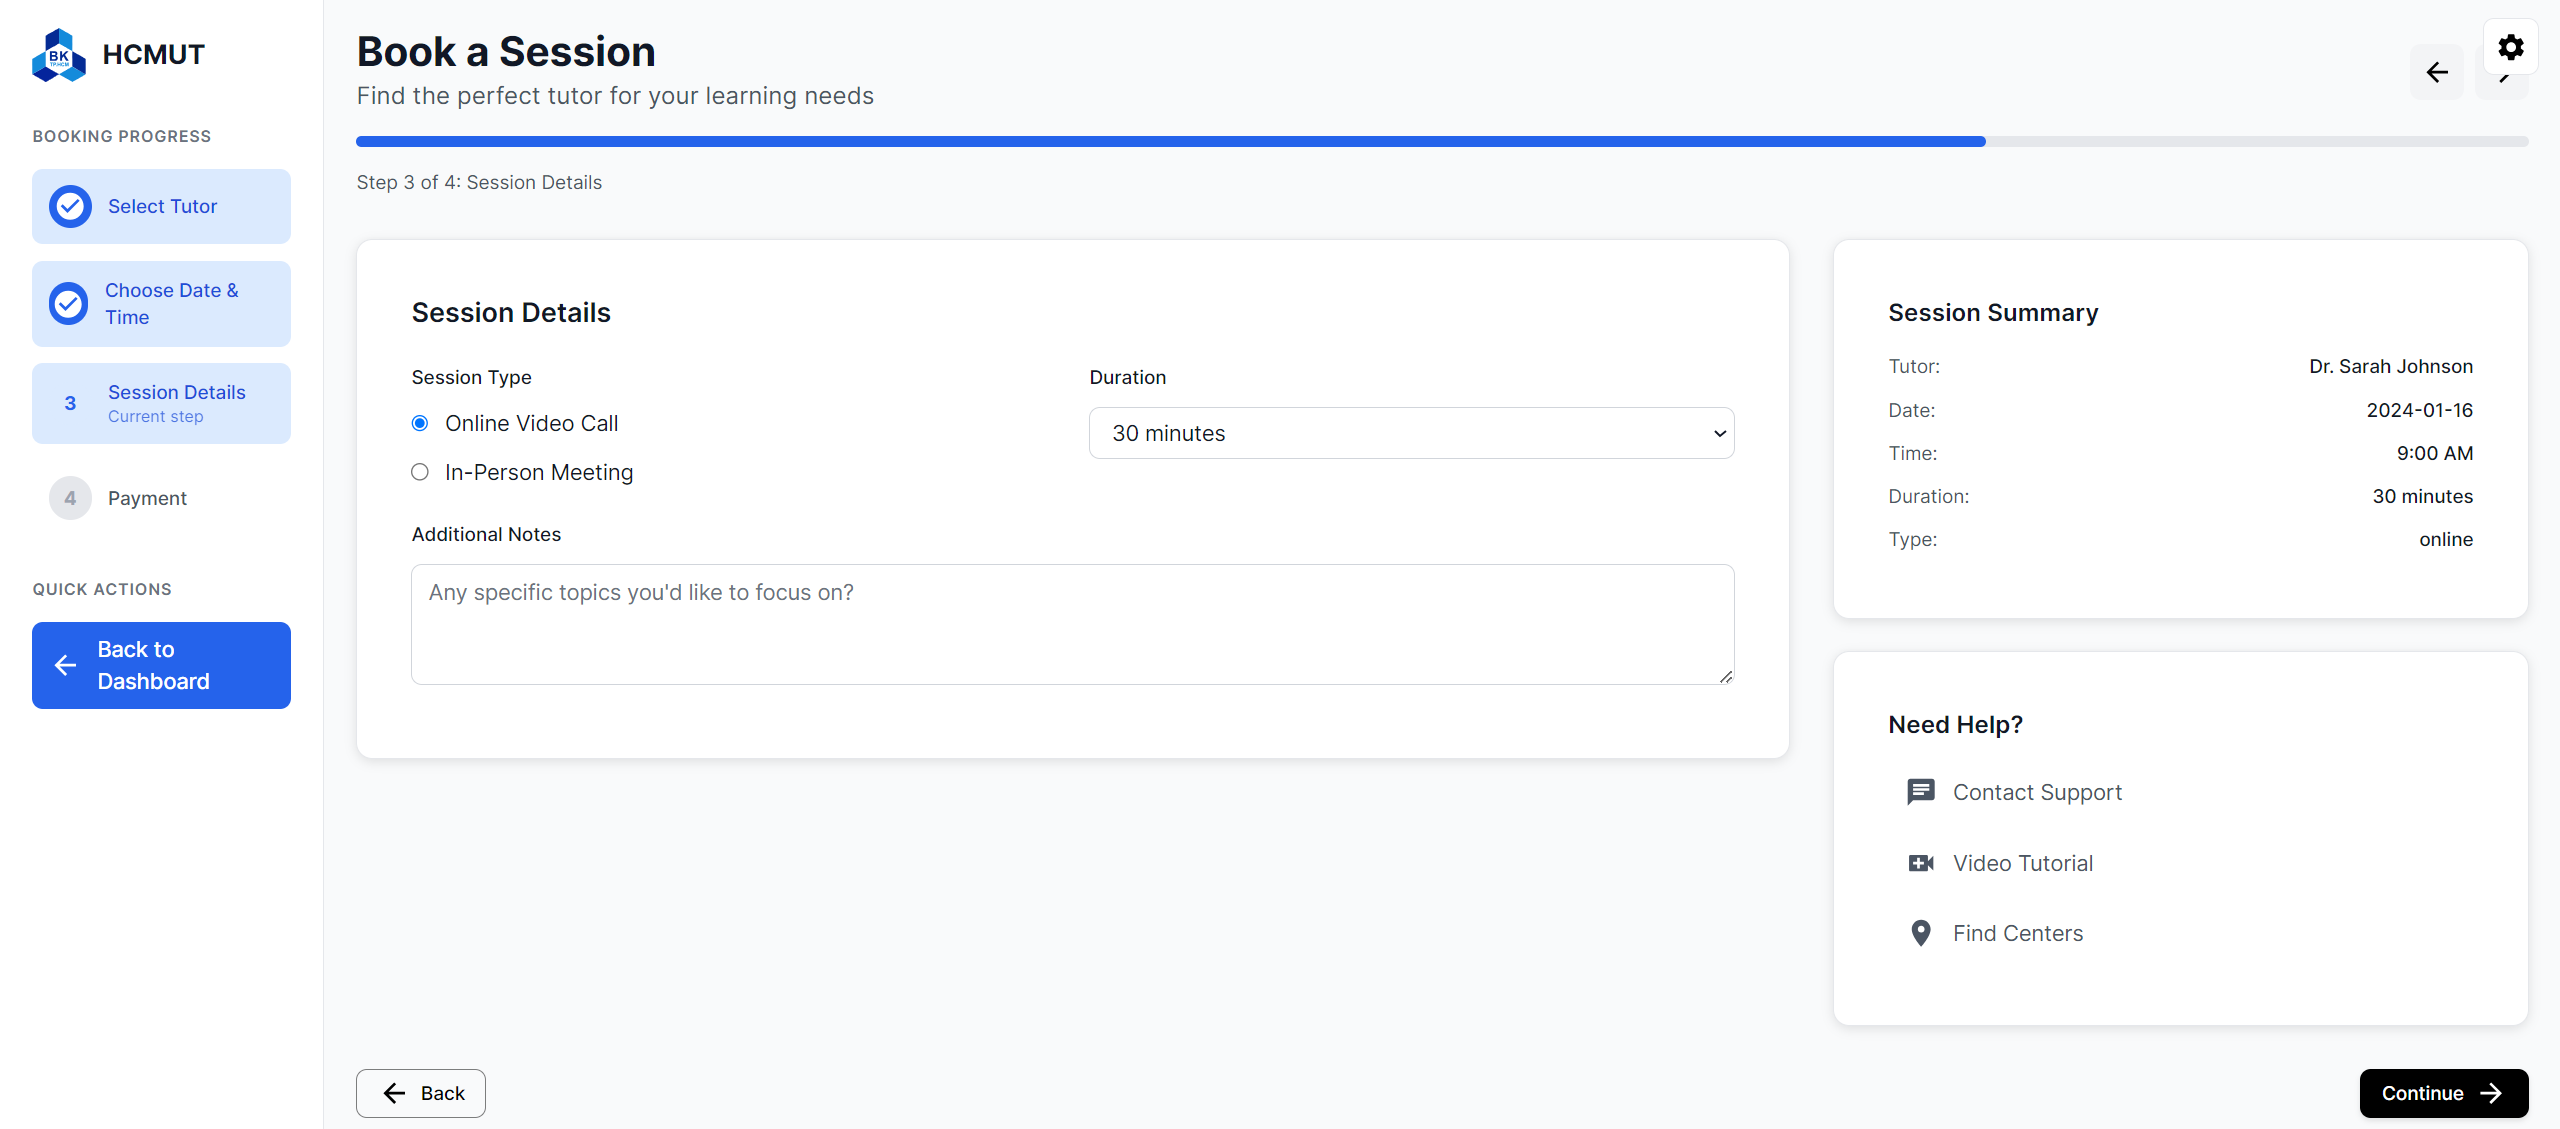
\includegraphics[width=\textwidth]{graphics/chapter2/student/book_session_step3.png}
    \caption{Book Session - Step 3: Session Details}
    \label{fig:book_session_step3}
\end{figure}

\paragraph{Step 3: Session Details}
The third step allows students to configure session specifics including session type (Online Video Call or In-Person Meeting), duration selection, and additional notes for the tutor. This ensures all session requirements are clearly communicated.

\begin{figure}[H]
    \centering
    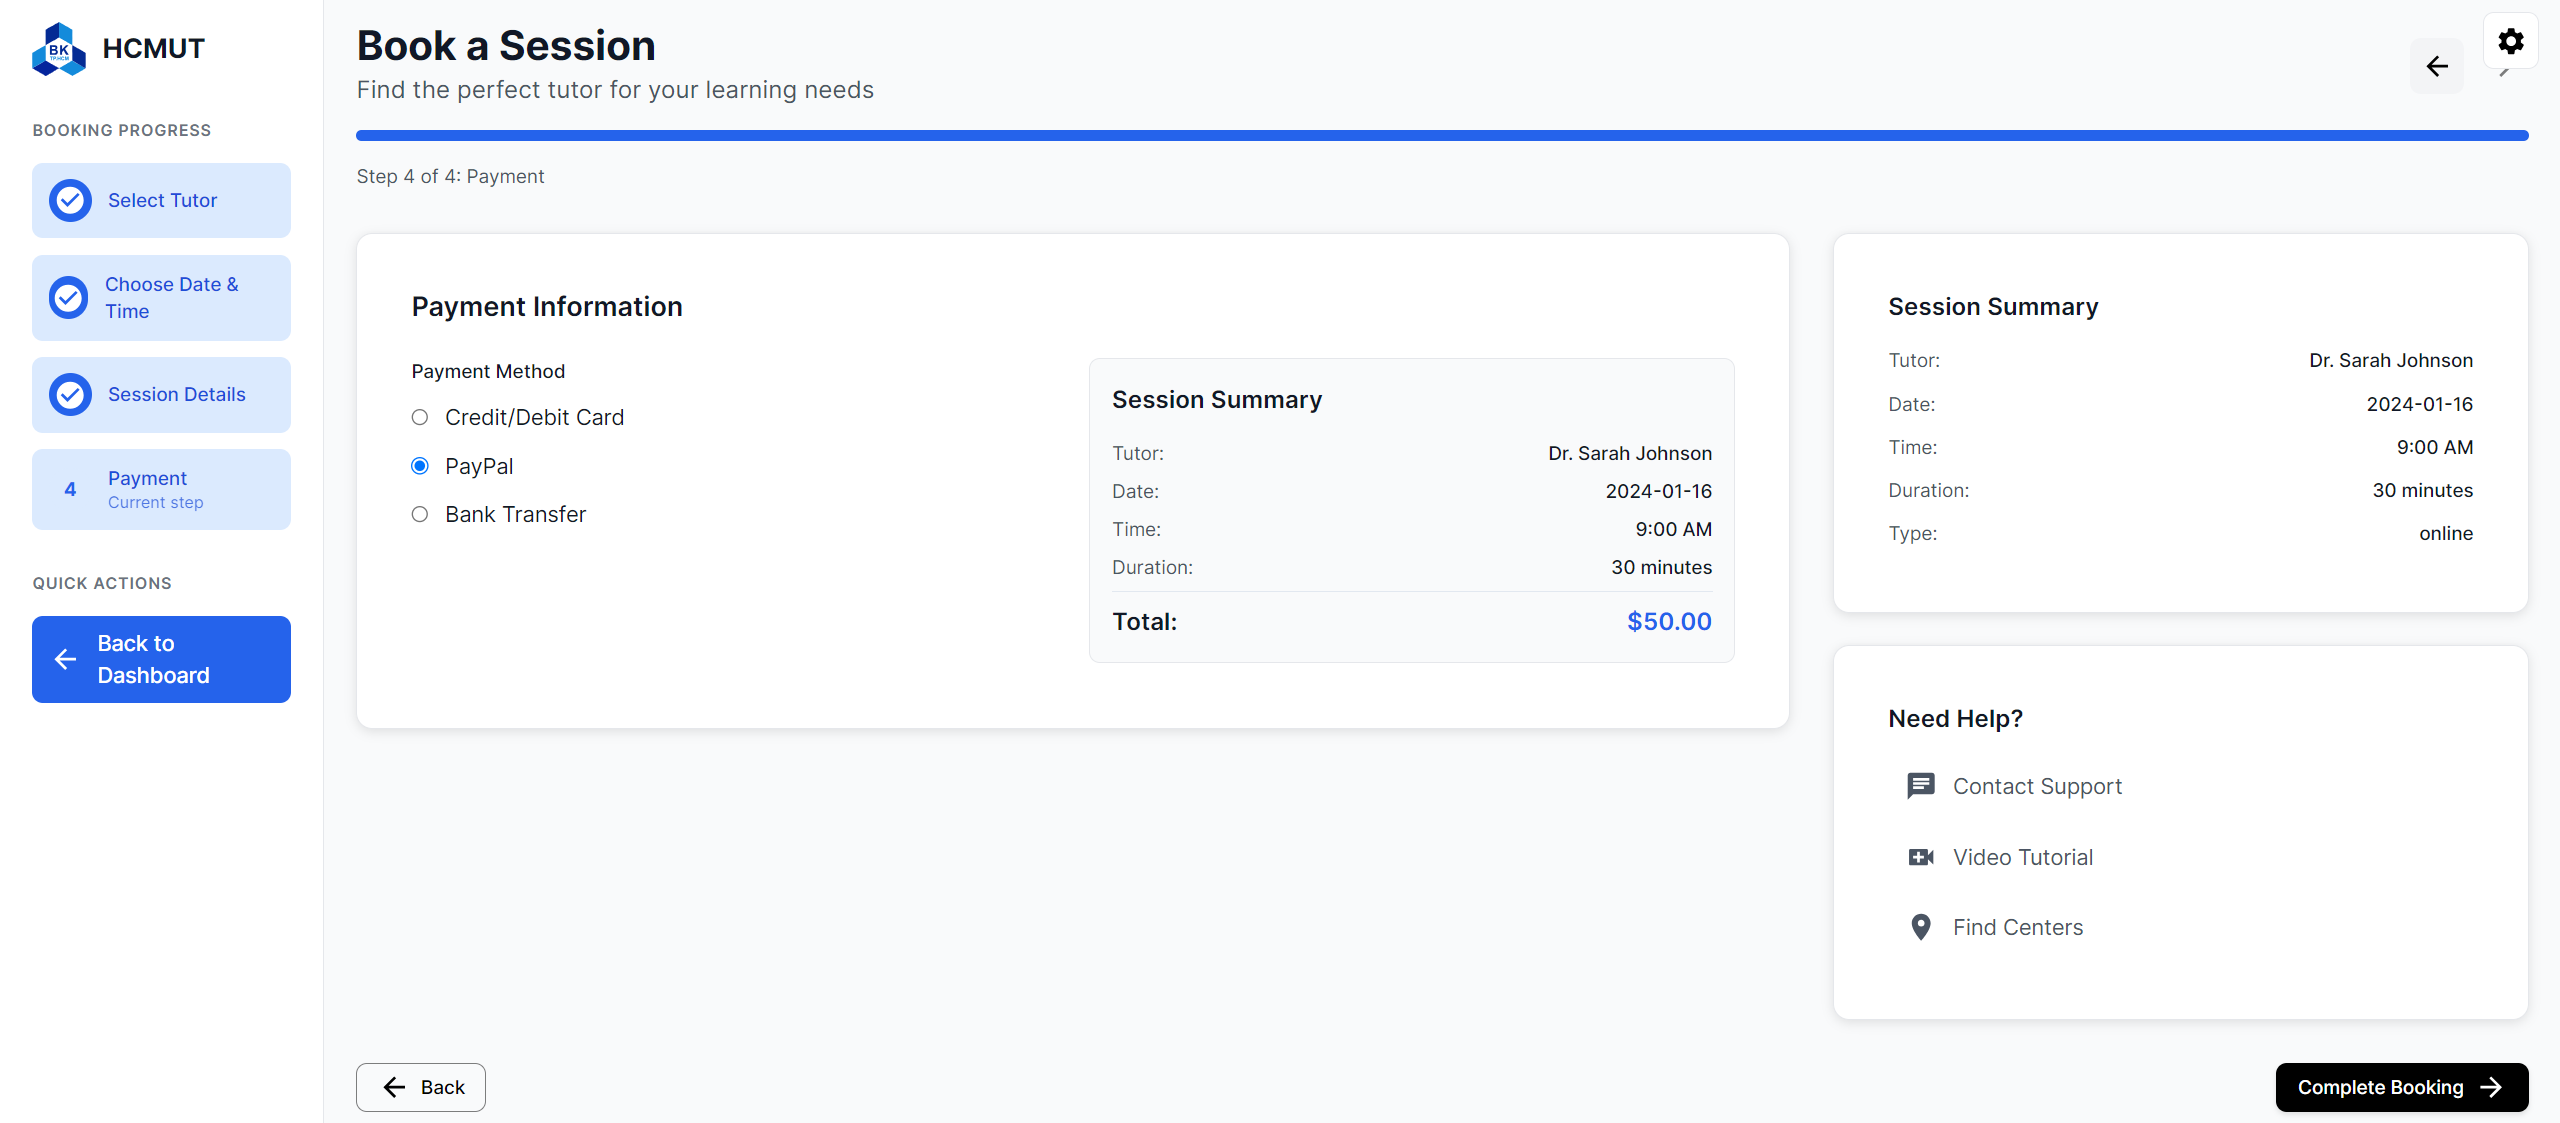
\includegraphics[width=\textwidth]{graphics/chapter2/student/book_session_step4.png}
    \caption{Book Session - Step 4: Payment (Mock)}
    \label{fig:book_session_step4}
\end{figure}

\paragraph{Step 4: Payment (Mock Implementation)}
The final step presents payment options including Credit/Debit Card, PayPal, and Bank Transfer. \textbf{Note: This payment section is implemented as a mock-up for demonstration purposes only, as this is a university project and does not involve actual financial transactions.} The interface displays session summary with total cost and provides navigation to complete the booking process.

\begin{figure}[H]
    \centering
    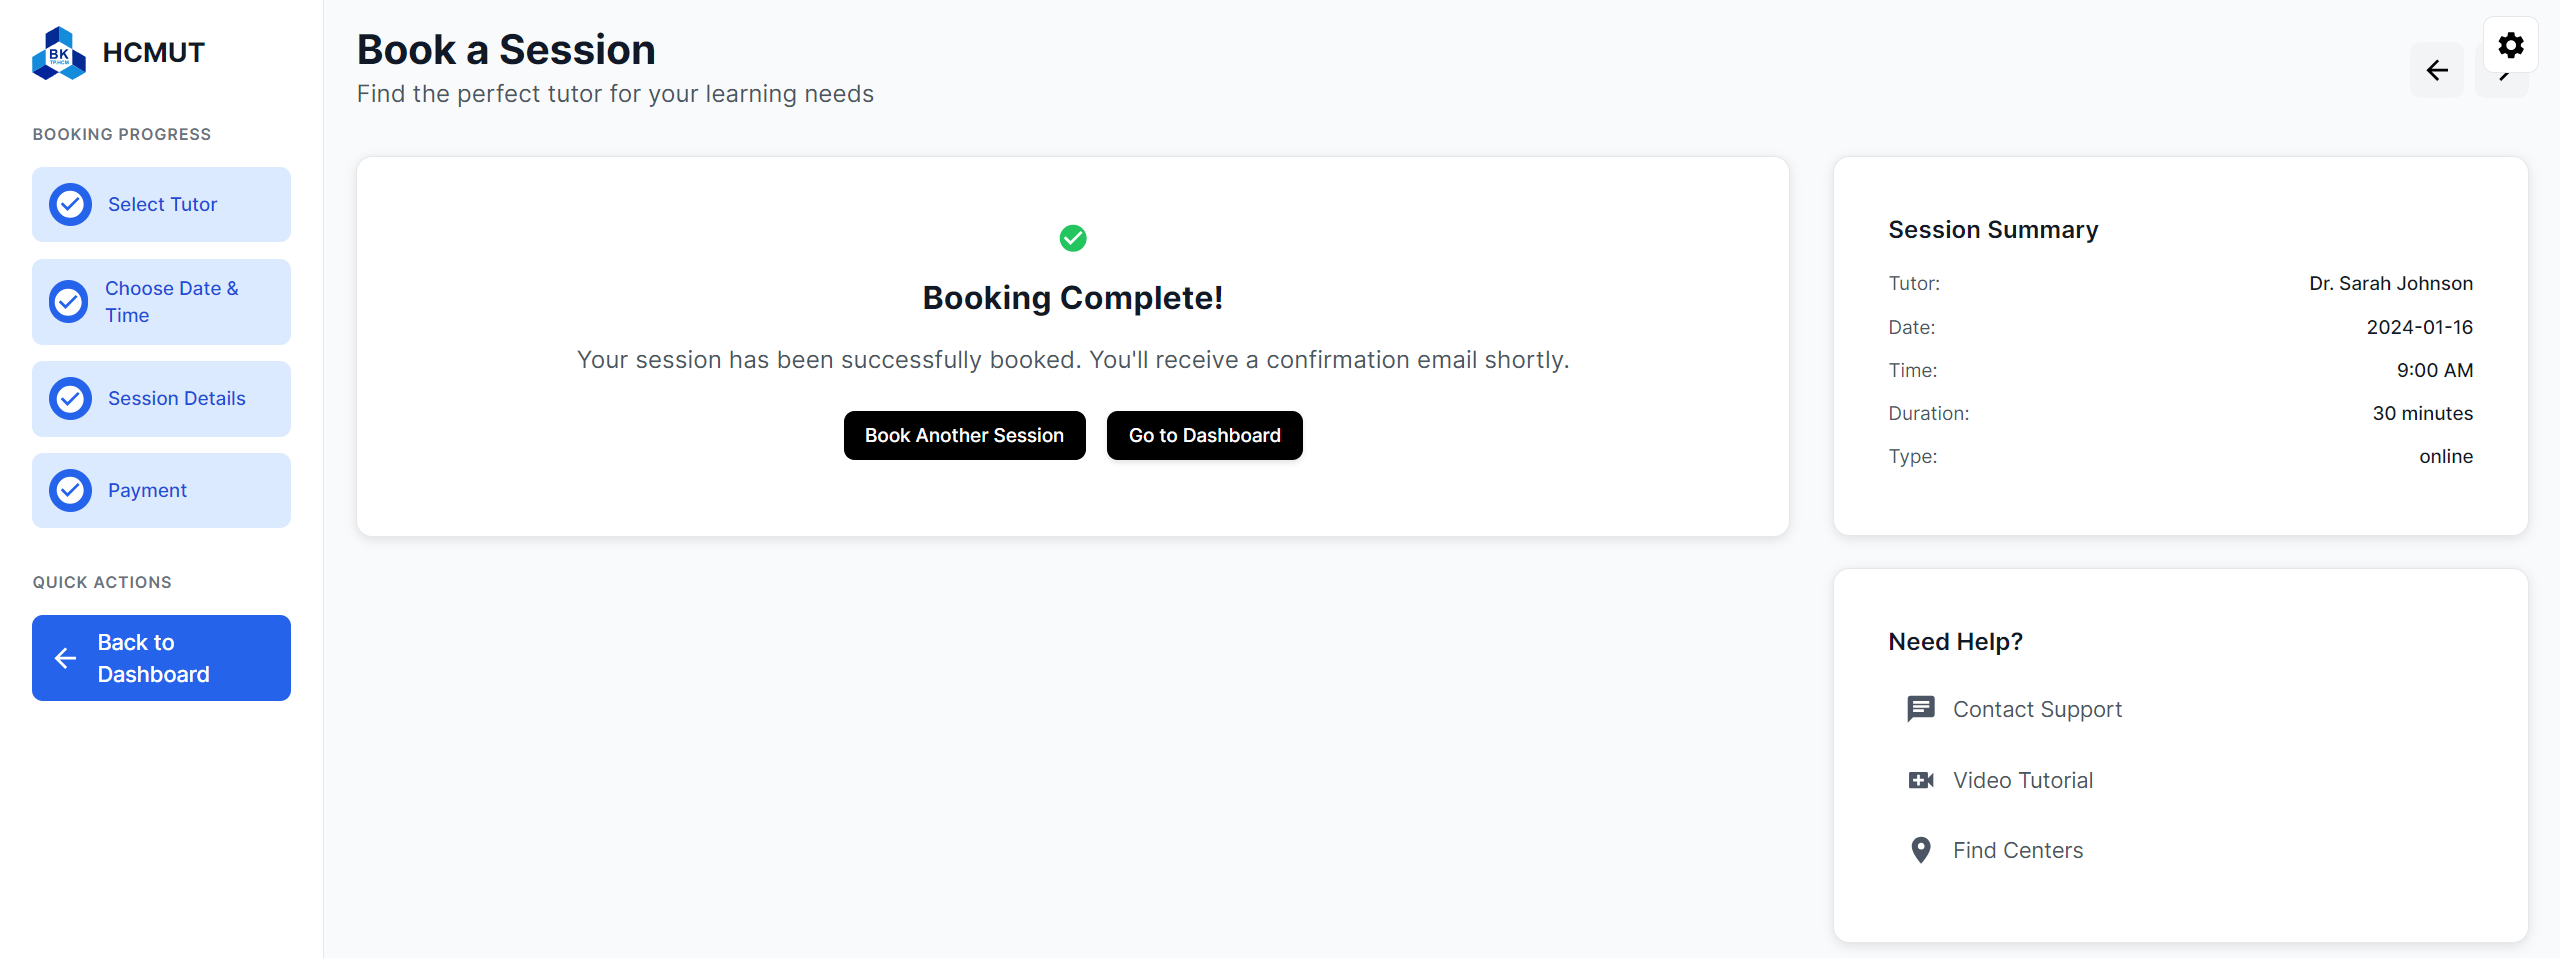
\includegraphics[width=\textwidth]{graphics/chapter2/student/book_session_complete.png}
    \caption{Book Session - Booking Complete}
    \label{fig:book_session_complete}
\end{figure}

\subsubsection{Session Detail}

\noindent The "Session Detail" page provides a comprehensive overview of a specific tutoring session, allowing students to view session information, tutor details, and access various actions related to the session.

\begin{figure}[H]
    \centering
    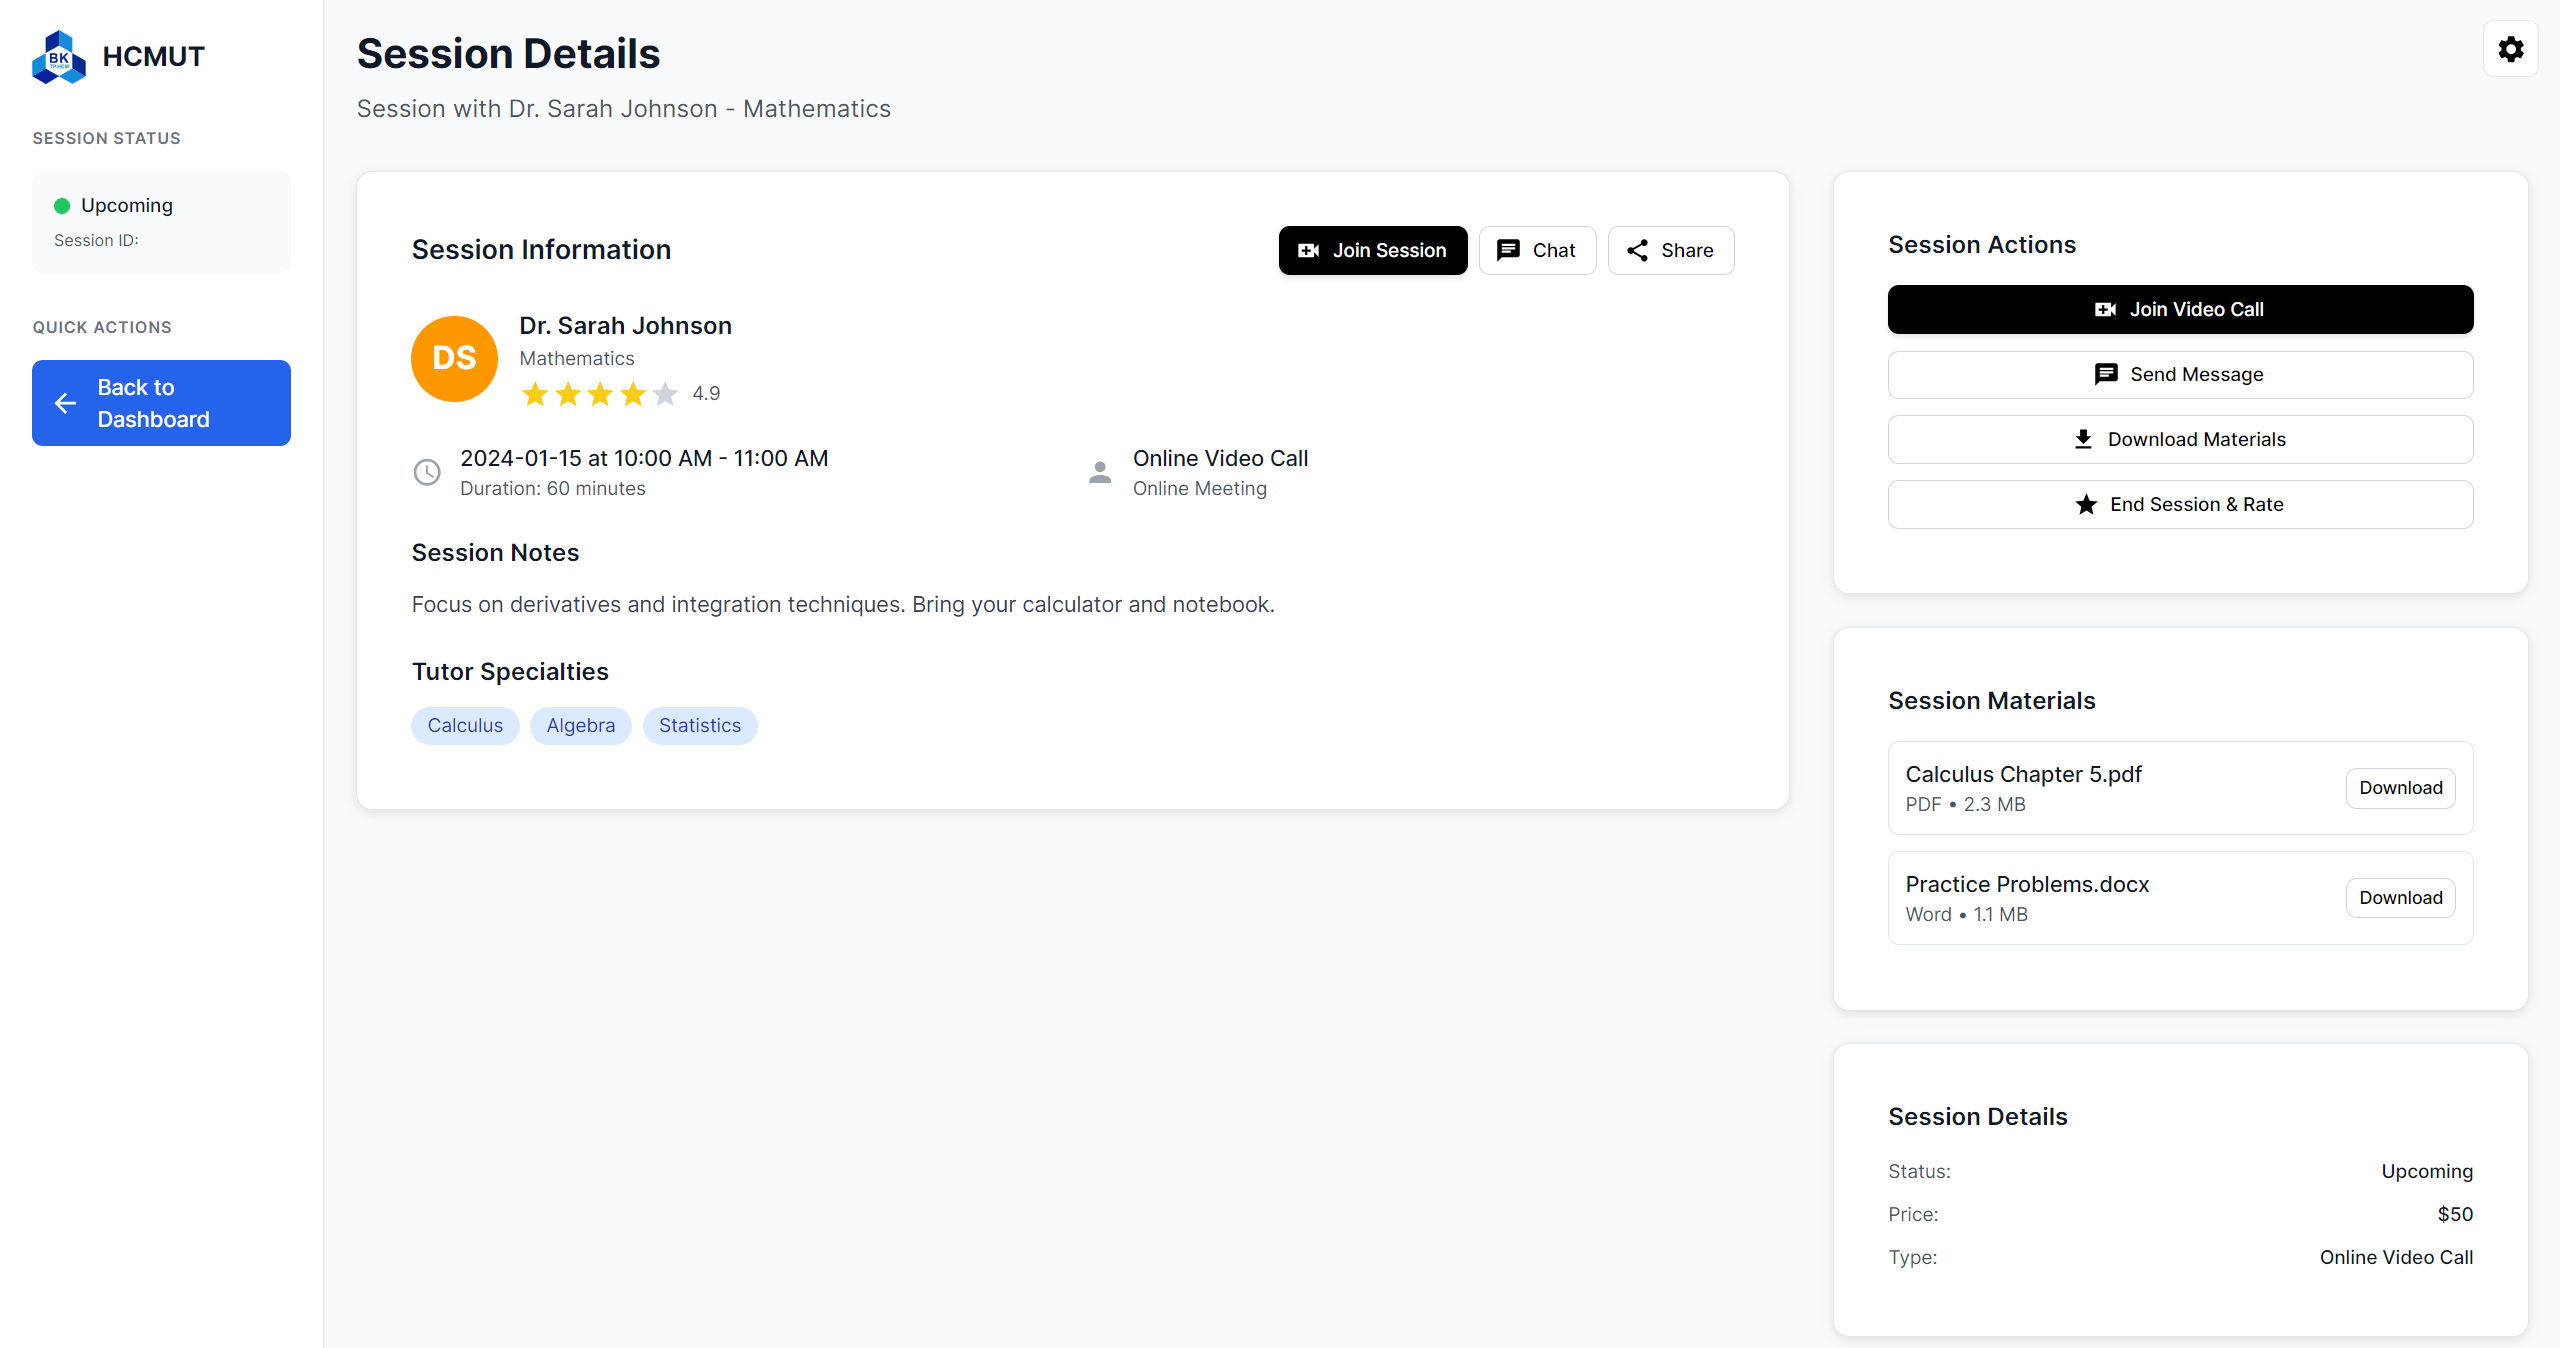
\includegraphics[width=\textwidth]{graphics/chapter2/student/session_detail_desktop_overall.png}
    \caption{Session Detail Page Overview (Desktop)}
    \label{fig:session_detail_desktop_overall}
\end{figure}

\paragraph{General Overview (Desktop)}
The desktop interface features a three-column layout with session information in the center, tutor details, session schedule, meeting type, session notes, tutor specialties, and action buttons for joining, chatting, sharing, and downloading materials.

\subsubsection{Evaluate Session}

\noindent The "Evaluate Session" page allows students to provide feedback on their tutoring sessions, rating various aspects of the session and the tutor's performance.

\begin{figure}[H]
    \centering
    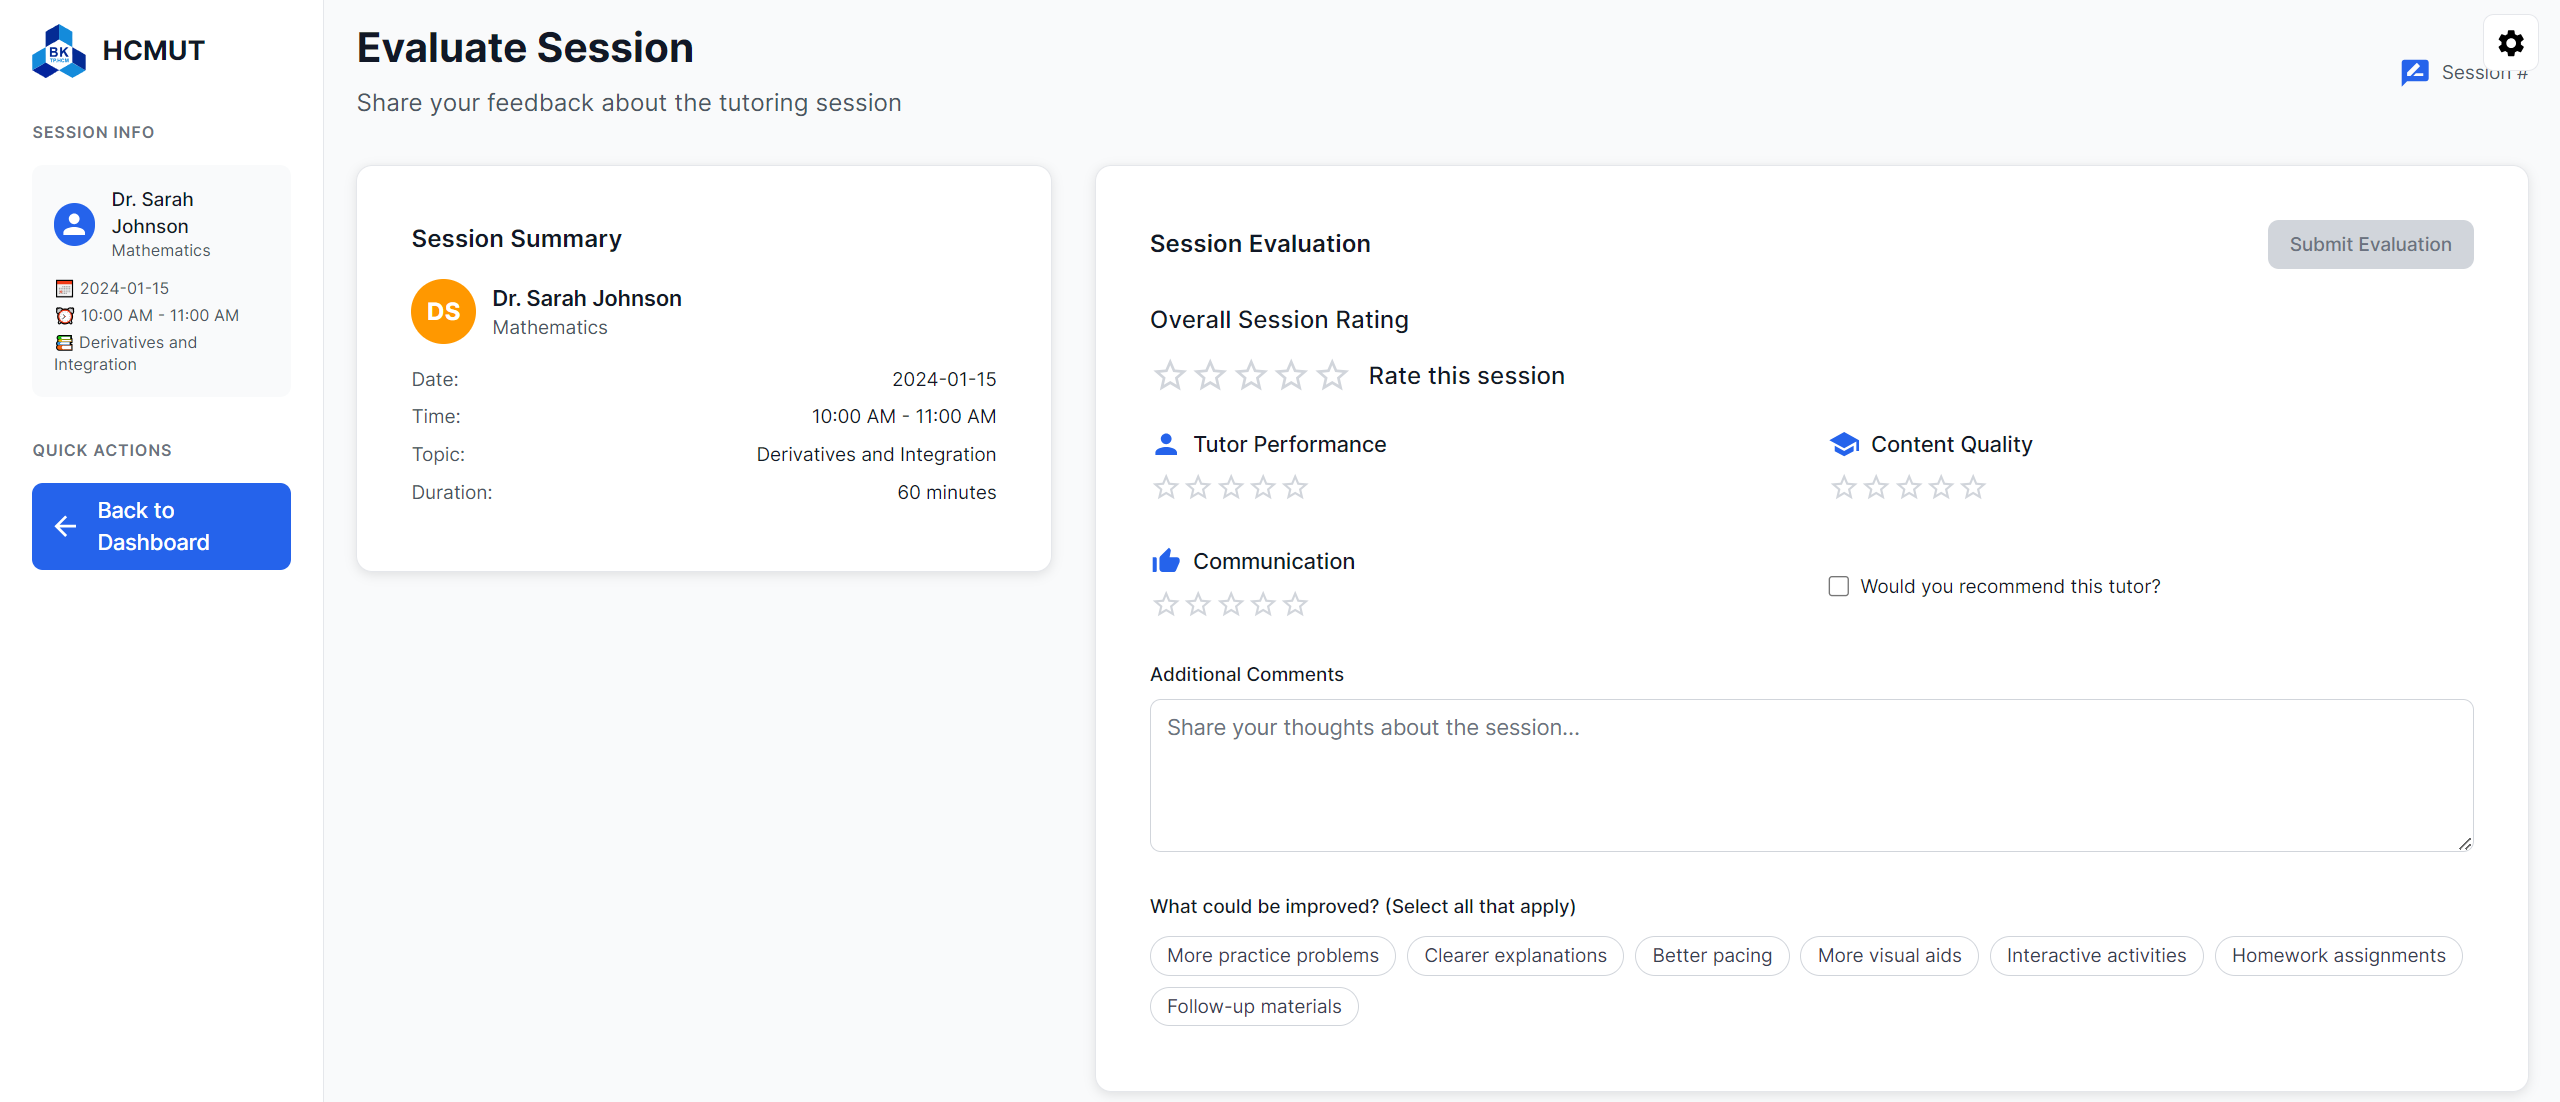
\includegraphics[width=\textwidth]{graphics/chapter2/student/evaluate_session_desktop_overall.png}
    \caption{Evaluate Session Page Overview (Desktop)}
    \label{fig:evaluate_session_desktop_overall}
\end{figure}

\paragraph{General Overview (Desktop)}
The desktop interface features a clean, card-based layout with session summary, rating system, feedback form, and improvement suggestions.

\subsubsection{View Progress}

\noindent The "View Progress" page provides students with a comprehensive overview of their learning journey, including overall progress, subject-specific performance, learning goals, and recent session activities.

\begin{figure}[H]
    \centering
    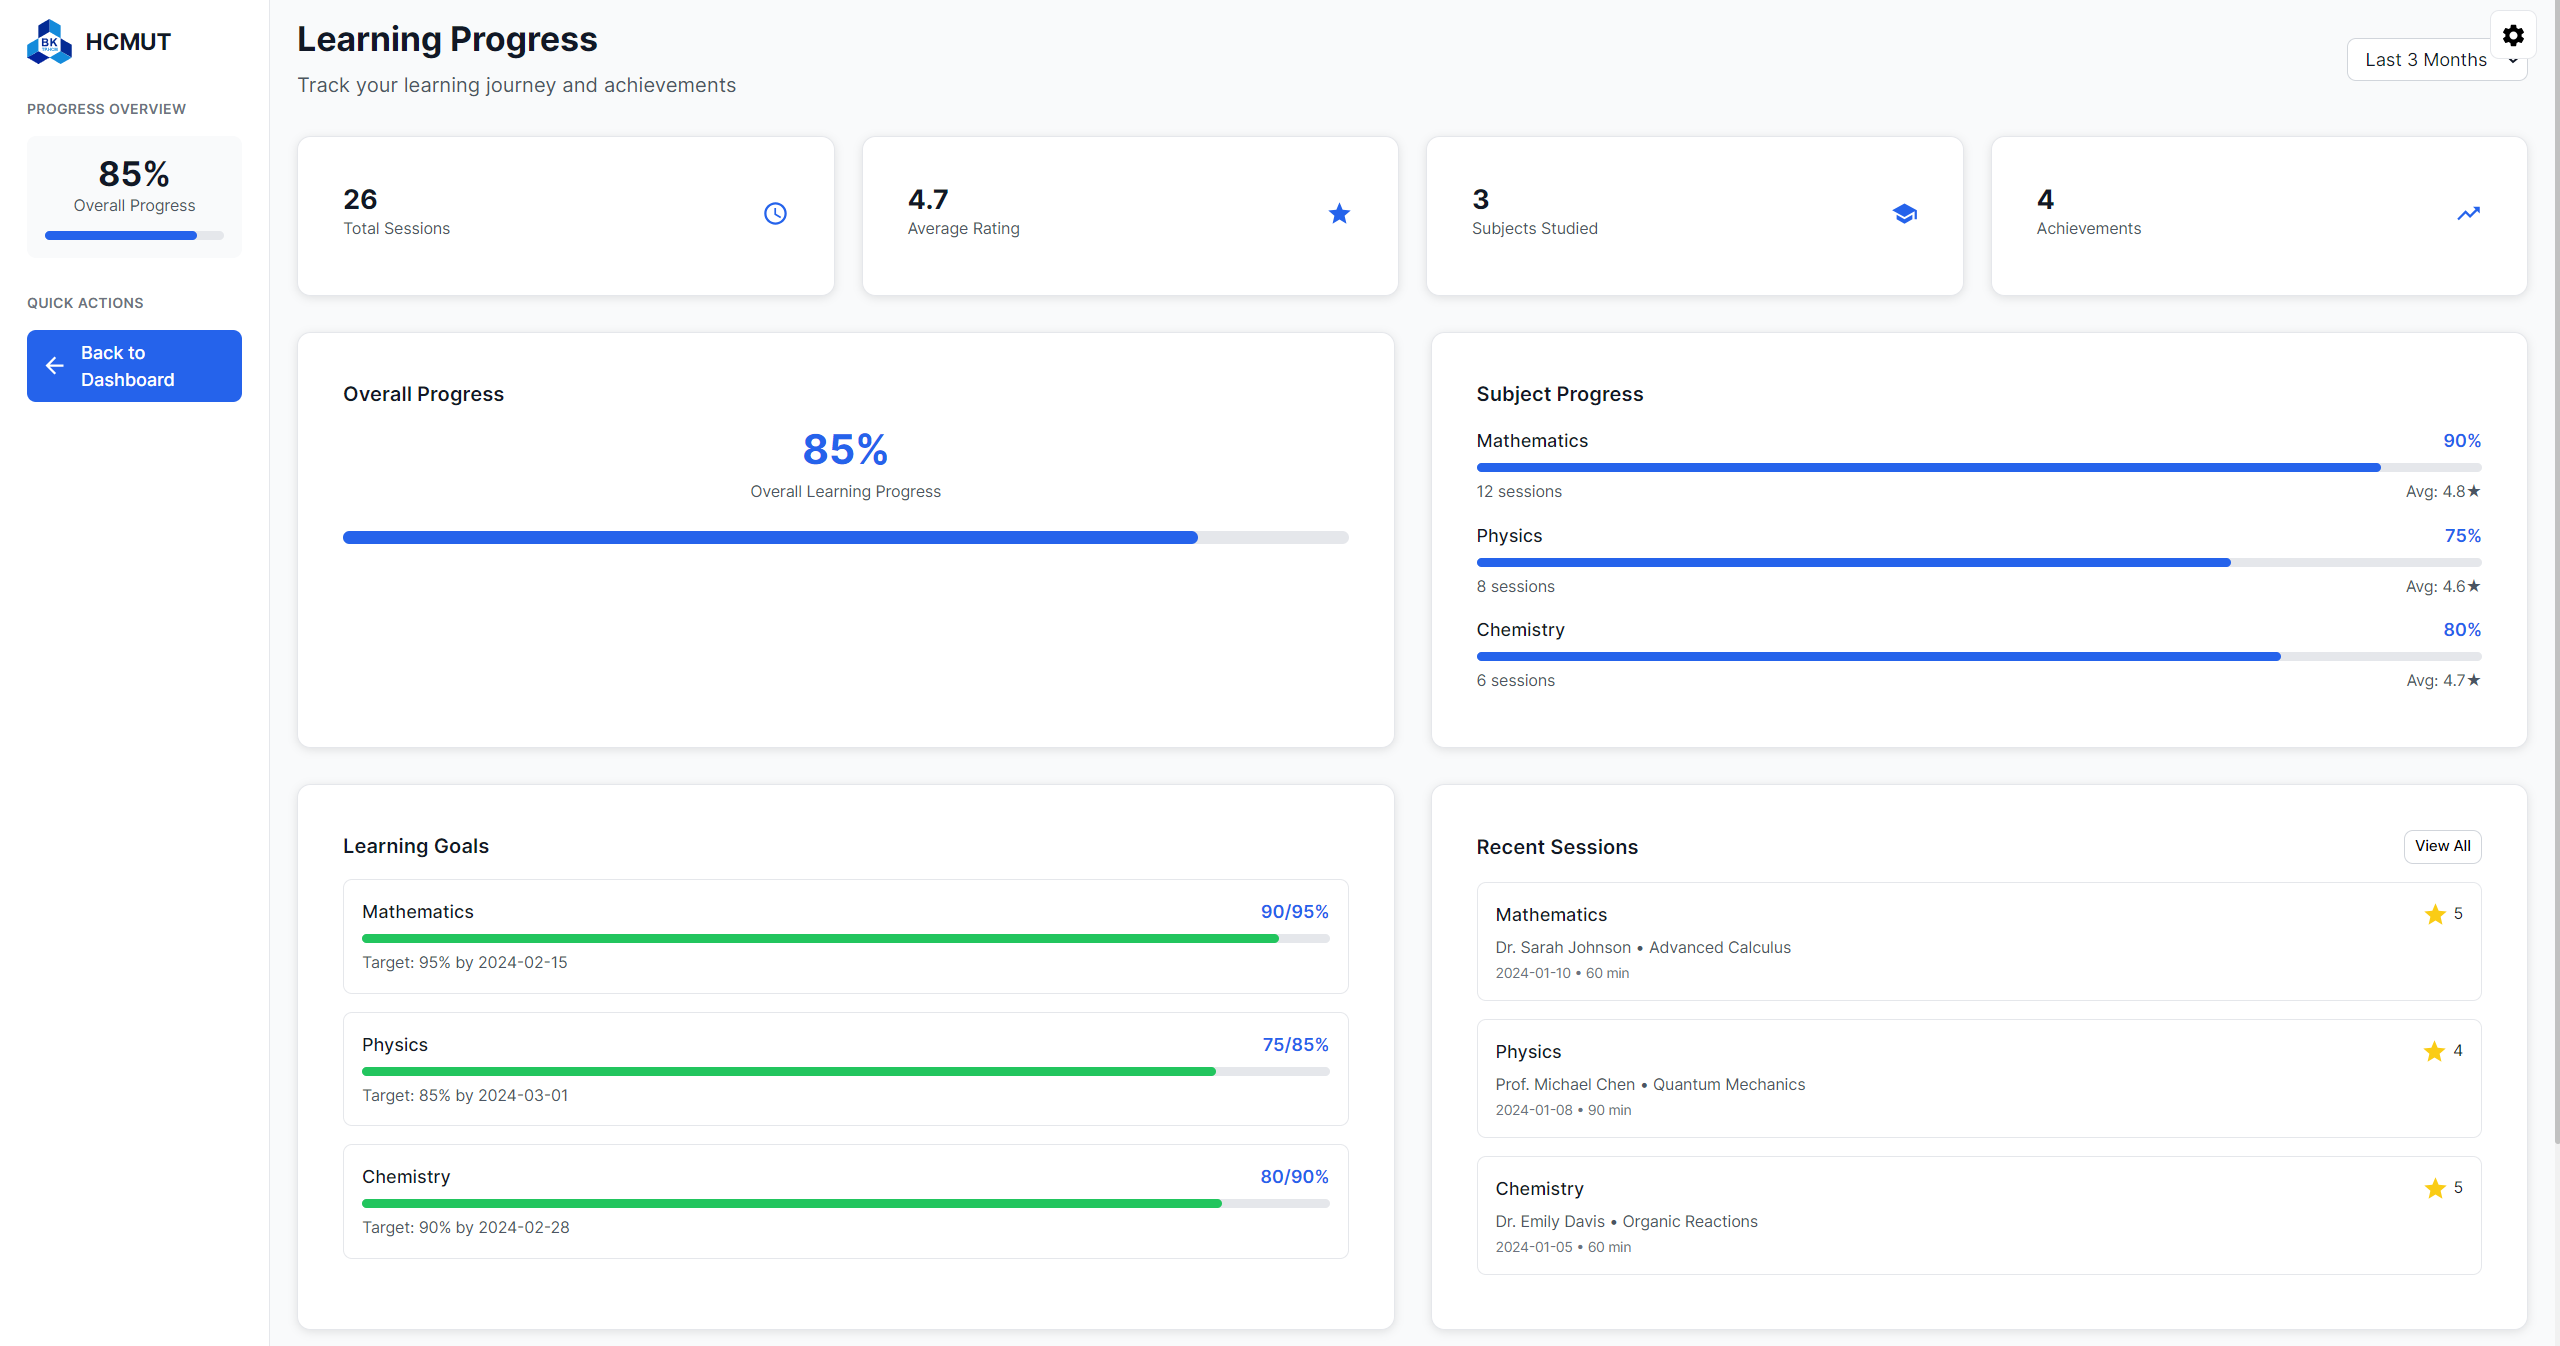
\includegraphics[width=\textwidth]{graphics/chapter2/student/view_progress_desktop_overall.png}
    \caption{View Progress Page Overview (Desktop)}
    \label{fig:view_progress_desktop_overall}
\end{figure}

\paragraph{General Overview (Desktop)}
The desktop interface features a clean, modern design with a three-column layout. The left sidebar provides progress overview and quick actions, while the central content area displays key metrics, learning goals, and subject progress. 

\subsubsection{Chatbot Support}

\noindent The "Chatbot Support" page provides students with an AI learning assistant for instant help with their studies, along with quick access to common support functions and FAQs.

\begin{figure}[H]
    \centering
    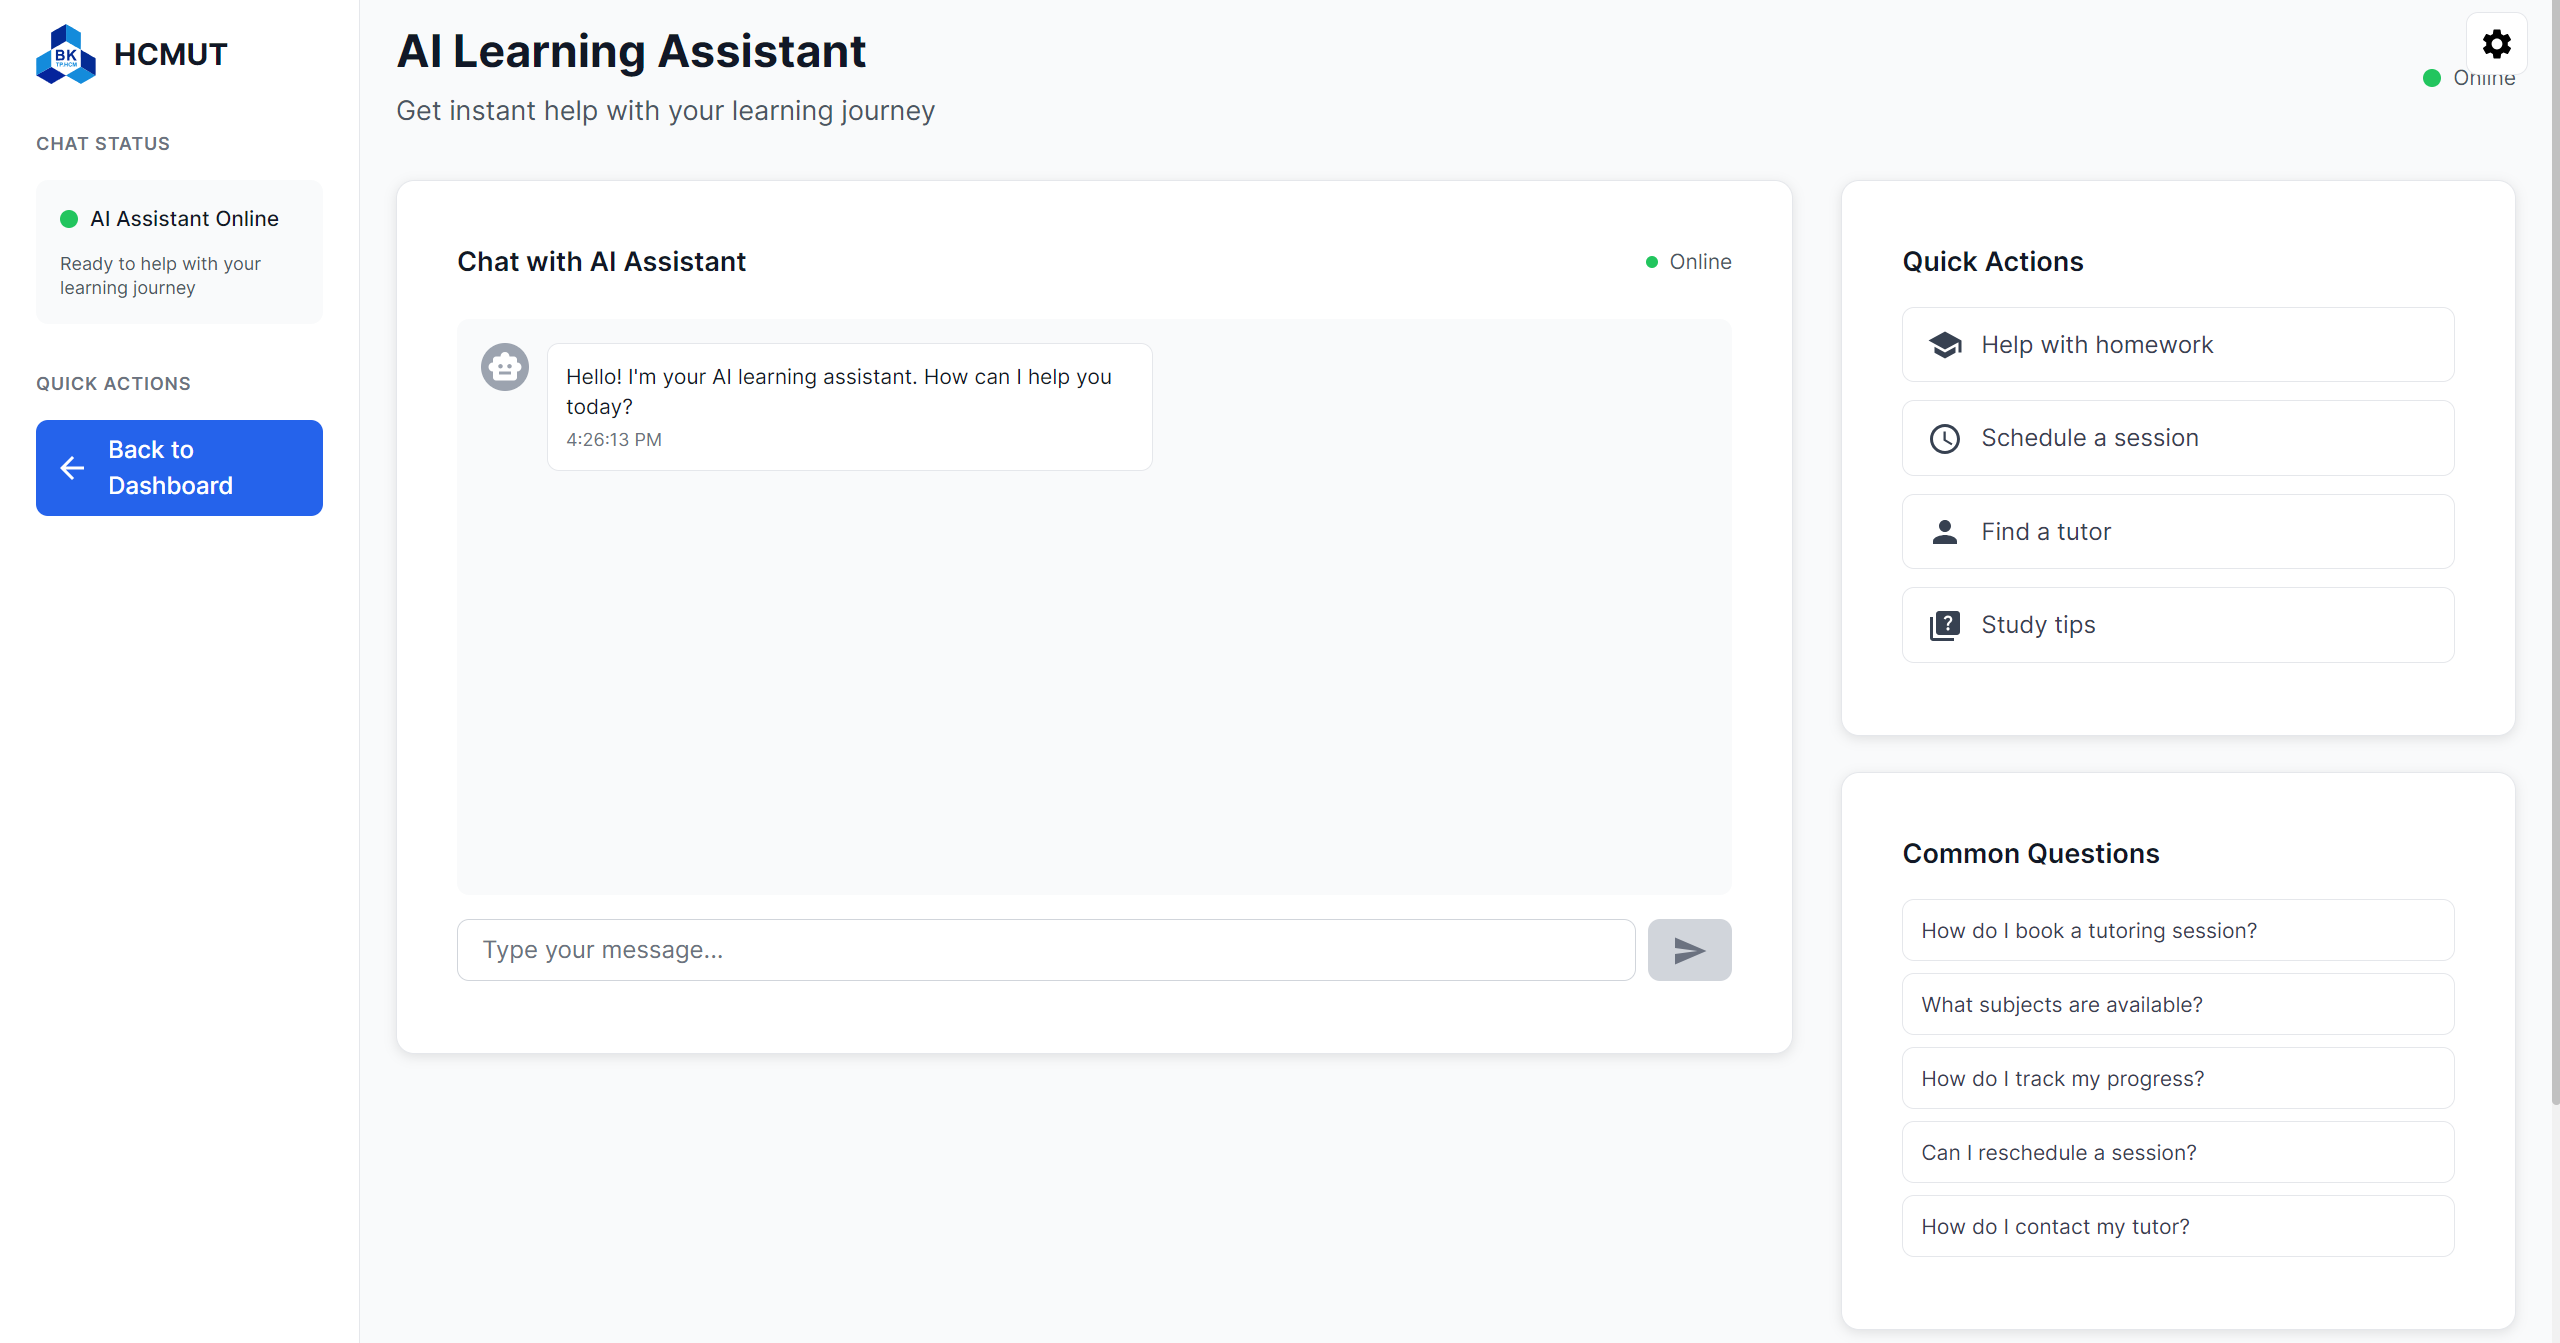
\includegraphics[width=\textwidth]{graphics/chapter2/student/chatbot_support_desktop_overall.png}
    \caption{Chatbot Support Page Overview (Desktop)}
    \label{fig:chatbot_support_desktop_overall}
\end{figure}

\paragraph{General Overview (Desktop)}
The desktop interface features a clean, two-column layout with the main chat interface and support options. 
